\section{Theory}
%Her skal jeg CARS (CREATE A RESEARCH SPACE) Presenter forskningsområdet («establish territory») Presenter tema og kunnskapsstatus i feltet
In order for my single-board computer to be able to extract useful information from the digital images it receives, it has to use fundamentals from image processing and mapping theory together to create a complete mapping system. There are also some requirements in terms of the processing power in the single-board computer, and to be able to run the mapping algorithm in a timely manner, these needs to be met. \\

The following section presents the theoretic basis for image processing and mapping, some sensor theory, as well as the requirements on the single-board computer. The theory section will share many similarities with the project report\cite{kris} I wrote fall of 2016 for Tor Onshus. The same fundamentals are being used in this thesis, but in terms of implementation; they vary. The theory section will focus on the theory for the techniques actually employed in the implementation, and less on presenting all the available techniques and selecting which ones to implement.\\

About half of the theory needed in this thesis is excerpt from Bjørnsen 2016\cite{kris}.


\subsection{Ground Sample Distance - GSD}
%se litt på
In order to associate image properties with real life properties of the mapping object, I can use what is known as Ground Sample Distance. When analyzing an image, this is a way to express and measure what one pixel in the image represents in real world units. The result will be a scaling factor given in $[m/pixel]$, where this factor can be used to scale pixel values to meter values.\\

Ground Sample Distance can be viewed as a measure of resolution limitations of an image sensor due to sampling\cite{s}. With the assumption that the sensor is pointed normal to the ground, it is in effect a measure of the real world distance between two pixels on the ground. The angular distance between sensor samples is given by pixel pitch $p$ divided by focal length of the sensor $f$. Assuming this angular distance is projected normal to the ground, it defines GSD:

\begin{align}
    GSD = \frac{p}{fW}R \quad\quad\textrm{[meters/pixel]}
    \label{gsd1}
\end{align}

\begin{figure}[H]
  \centering
  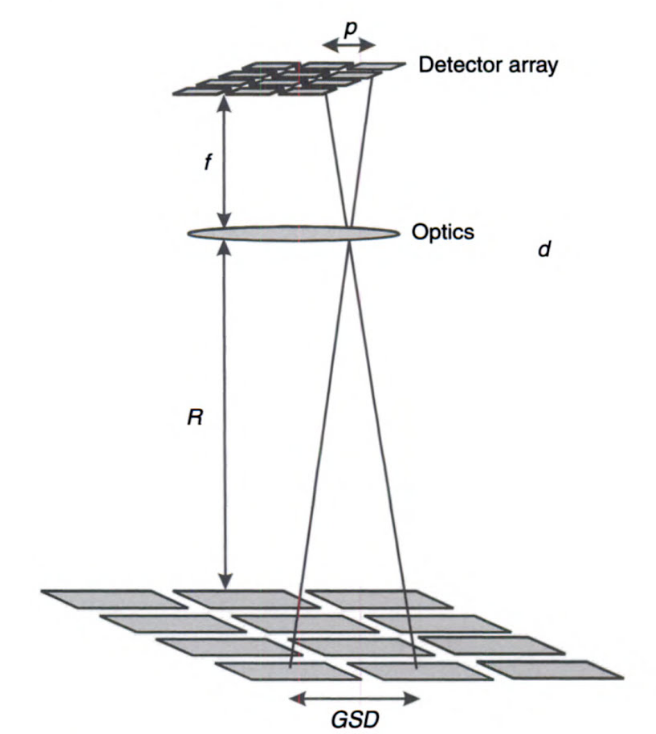
\includegraphics[width=0.7\textwidth]{fig/GSDimage}
  \caption{Ground Sample Distance. From \cite{s}}
  \label{fig:gsd}
\end{figure}


Where $R$ is the distance from the optics to the ground and $W$ is the width of the image in pixels. GSD is illustrated in Figure \ref{fig:gsd}. Equation \ref{gsd1} assumes that the sensor is directed normal to the ground surface. If the sensor is not aligned normal to the ground, the GSD must be expanded for the look angle between the ground and the sensor $\theta$:
\begin{align}
    GSD = \frac{pR}{fW\cos{\theta}}\quad\quad\textrm{[meters/pixel]}
    \label{gsd2}
\end{align}
Where $\theta$ is the angle the sensor is facing with respect to the ground plane. By taking the geometric mean of the horizontal and vertical ground sample distances you get a two-dimensional system GSD\cite{s} factor. \\

To calculate GSD it is assumed that certain camera properties are known and that we have a way to measure or calculate the distance from the object to which we are calculating the GSD. With these pieces of information, it is possible to convert an image from pixels to real life units.
\newpage
\subsection{Image Processing}
%FERDIG
The digital camera is a powerful sensor that has many provides many advantages in technical applications and implementations. It is a sensor that can be used for the identification of environmental variables within the line of sight, and can easily be combined with other sensors. Many autonomous applications employ cameras, and together with image processing it provides a powerful tool to automate advanced tasks and real life objectives. Self-driving cars\cite{tesla} use cameras as well as other sensors to extract useful information from the environment.\\

As an example, in a self-driving car application, one might be interested in determining the size and location of other cars on the road in order to prevent collisions and provide an autonomous driving experience. Image processing is a topic that can be related to several fields of engineering, from simple automation to complex artificial intelligence.\\

In the following section I will present the fundamental underlying theory of edge detection and some of the image processing methods I use in my thesis.
%--------------

\subsubsection{Edge Detection}
%Omskrive litt
A powerful tool to use when trying to identify the characteristics of a the environment is edge detection. Edge detection is based on detecting sharp, local changes in intensity in an image. At a fundamental level, abrupt, local changes in intensity can be detected by using derivatives, where first- and second order derivatives are the most used \cite{g}. \\

Figure \ref{fig:derivatives} illustrates the differences between the intensity response of the first- and second order derivatives on an edge with a ramp response.

\begin{figure}[h]
  \centering
  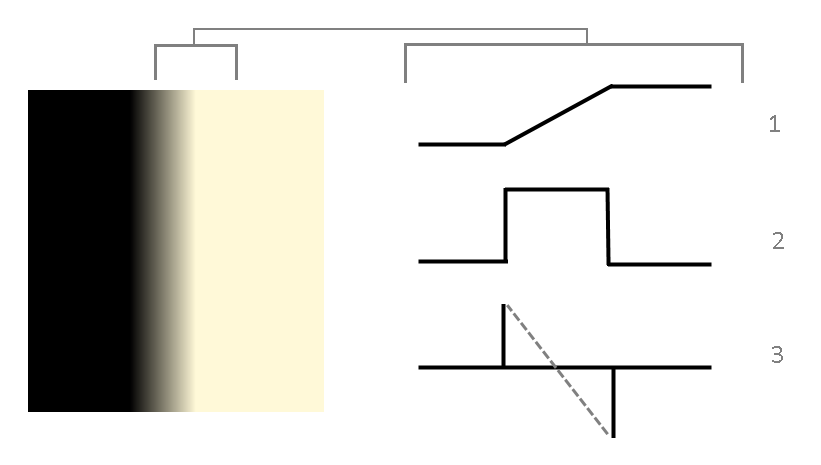
\includegraphics[width=0.8\textwidth]{fig/derivatives}
  \caption{(1) Horizontal intensity profile. (2) First derivative. (3) Second derivative with zero crossing}
  \label{fig:derivatives}
\end{figure}

\subsubsection{Edge Detection methods based on first derivatives}
%Omskrive litt
As mentioned previously, edges are characterized as a change in intensity in an image. Digital images are discrete, therefore we have to use an approximation of the first derivative with the requirements that; (1) it must be zero in areas of constant intensity, (2) it must be nonzero at the onset of an intensity step or ramp, and that (3) it must be nonzero at points along an intensity ramp\cite{g}. It is important to note that most edges in an image does not change its value immediately, but tends to change more gradually, like a ramp-function. Our requirements covers this, where the derivative must be non-zero along an intensity ramp.\\
We first consider the one-dimensional function $f(x)$, we approximate by Taylor expansion about $x$ of $f(x+\Delta x)$, where we let $\Delta x = 1$, and keep the linear terms:
\begin{align}
    \frac{\partial f}{\partial x} = f'(x) = f(x +1) - f(x)
\end{align}
We used the partial derivative here because the image is a function of two variables. We approximate the the derivative by Taylor expansion in the $y$ dimension just like we did above:
\begin{align}
\frac{\partial f(x,y)}{\partial x} = f(x+1,y)-f(x,y) = g_x\\
\frac{\partial f(x,y)}{\partial y} = f(x,y+1)-f(x,y) = g_y
\end{align}
A powerful tool in edge detection is to define the gradient, $\nabla f$ as
\begin{align}
\nabla f \equiv grad(f) \equiv 
\begin{bmatrix}
g_x \\
g_y
\end{bmatrix}
= 
\begin{bmatrix}
\frac{\partial f}{\partial x}\\
\frac{\partial f}{\partial y}
\end{bmatrix}\\
M(x,y) = \sqrt[]{g_x^2 +x_y^2}
\label{eq:magnitude}
\end{align}
Where the $\nabla f$ vector gives us information about the edge strength as well as the direction of the greatest rate of change of $f$ at location $(x,y)$.\\

The direction of the edge can be expressed as:
\begin{align}
\alpha(x,y) = \arctan(g_y/g_x)
\label{eq:direction}
\end{align}

Obtaining the gradient of an image involves calculation the partial derivatives $\frac{\partial f}{\partial x}$ and $\frac{\partial f}{\partial y}$ at every location of the pixels in the image. In order to do this we use spatial filtering in the image (also known as masking). The process of spatial filtering consists of moving a filter mask from point to point in an image, and calculating the filter response of the original image at each point $(x,y)$ in the image. The filter values are pre-defined and characteristics of the filter can be modified in order to achieve different improvements in an image such as image enhancement.\\

We want to look for edges in two dimensions; x and y direction, thus the most used edge detection algorithms use 2D spatial filters to find edges. A general 3x3 spatial filter mask can be represented as a table of intensity values $z_i$ as illustrated in Table \ref{spatial}.
\begin{table}[h]
\centering
\caption{General 3x3 Spatial Filter Mask}
\label{spatial}
\begin{tabular}{|l|l|l|}
\hline
$z_1$ & $z_2$ & $z_3$\\ \hline
$z_4$ & $z_5$ & $z_6$\\ \hline
$z_7$ & $z_8$ & $z_9$\\ \hline
\end{tabular}
\end{table}

Edge detection methods based on the first derivative are generally more primitive than those based on the second order derivative. They are generally less computationally intensive, but offer limited functionality and robustness. For my application I will implement a method based on the second derivative.

\subsubsection{Edge Detection methods based on the second derivative}
%Skrive om at det er dette vi bruker i vår applikasjon
The requirements set on the approximation of the second order derivative is similar to that set on the first order derivative. The only difference is that I now only require the second order derivative to be non-zero at the onset and end of a ramp in intensity value. This means that the first order derivative methods will create "thicker" edges since its non-zero along the whole ramp, while the second order derivative methods will lead to "thinner" edges, since the values are non-zero only at the beginning and the end of a ramp.



\subsubsection{Canny edge detection method}
%endre litt, ikke "a different edge detection alg---"
A complex edge detection algorithm is the Canny edge detector\cite{canny}. In general, the Canny method is regarded as superior to most other edge detection algorithms, including other edge detector based on the second derivative, and is based on three objectives:
\begin{itemize}
\item Low error rate. The algorithm should find all the edges in an image, regardless or orientation. Should be as close as possible to the actual edges.
\item Edge points should be well localized. Detected edges should be close to the actual edges.
\item Single edge point response. Should not return multiple edge points where only a single edge point exist.
\end{itemize}
The Canny method starts with applying a Gaussian filter to convolve with the image in order to smooth out noise. After this the gradient magnitude (\ref{eq:magnitude}) and the direction (\ref{eq:direction}) are calculated:
\begin{align*}
M(x,y) = \sqrt[]{g_x^2 +x_y^2}\\
\alpha(x,y) = \arctan(g_y/g_x)
\end{align*}
After this it applies a non-maximum suppression technique to the gradient magnitude image which thins the edges. This helps suppress all the gradient values to zero except the local maximal, which is the the sharpest change in intensity value, thus fulfilling the objective of giving a single edge point response.\\

The last part of the algorithm is to use double thresholding to determine strong and weak edges. Edges with intensity values below the lowest threshold are suppressed, which is noise in most cases. This is a tuning parameter and needs to be determined empirically. The last step of the algorithm also involves tracking edges and conducting a connectivity analysis to detect and link edges together, where edges that are weak and not connected to strong edges are suppressed.\\

\newpage
%Skal jeg ha med dette?
\subsection{Image pre-processing before Edge detection}
There are a number of different techniques and methods one can employ before using an edge detection algorithm to get a better edge detection result.
\subsubsection{Correcting Nonuniform Illumination}
Depending on the lighting conditions in the image, it might be beneficial to correct for nonuniform illumination. This can be done in several ways, but the most normal being estimate the background illumination of the image, inverse it and subtract it from the original image.
\subsubsection{Smoothing}
Smoothing is beneficial to suppress noise in the image. This can be done by applying a Gaussian filter to the image, which described previously in some of the edge detection algorithms. Smoothing is a part of some of the edge detection algorithms, which is designed to suppress noise.
\subsubsection{Increase contrast}
Increasing contrast can help in the detection of edges in an image. This is done by saturating the top and bottom $1\%$ of intensity values in the image. In the implementation described later in the report, this is utilized to improve the edge detection algorithm.
\subsubsection{Re-sizing}
By re-sizing the image by a scale factor the image will be smoothed. Some edge detection algorithms work better with images that are scaled down and smoothed. This is described later in Section \ref{testing}, and how this affects edge detection and edge linking quality.
%-----------

\newpage
\subsection{Edge Linking}
%Skrive slik som vi gjør det i OpenCV
After the edge detection algorithm has been applied to the image, we ideally have detected all the edge pixels in the image perfectly. Most of the time, this is not the case. The edge detection is therefore followed up by edge linking, where we attempt to assemble edge pixels into meaningful edge segments. Since actual edges will have the property of being fully or partly connected straight lines, noise in the image will naturally be suppressed and not detected. 
%--------

\subsubsection{Hough Transform}\label{ch:hough}
%Skrive slik jeg gjør i opencv
The Hough transform is a global processing method of edge linking \cite{hough}.  Considering a point $(x_i,y_i)$ in the xy-plane, we can describe infinitely many lines running through this point as $y_i = ax_i + b$ for any $a$ and $b$. We can rewrite this as $b = -ax_i + y_i$, and consider the ab-plane, which is known as the parameter space. This gives an equation for a single line for a single xy-pair $(x_i,y_i)$. A different xy-pair $(x_j,y_j)$ also has a line expressed in parameter space $b = -ax_j + y_j$, and if the lines are not parallel, the lines will intersect at a point $(a',b')$. $a'$ is the slope, and $b'$ is the intercept of the line containing both $(x_i,y_i)$ and $(x_j,y_j)$. The points on this line will have lines in the ab-plane that intersects at $(a',b')$.\\

One fundamental problem representing lines on the form $y = ax + b$ is that $a$ approaches infinity as the line gets closer to vertical. It is therefore beneficial to represent the lines as:
\begin{align*}
x\cos{\theta} + y\sin{\theta} = \rho
\end{align*}
This is a transformation to the $\theta\rho$-plane, which is very similar to that of the ab-plane. $(\theta',\rho')$ corresponds to the line that passes through both $(x_i,y_i)$ and $(x_j,y_j)$. When $(\theta',\rho')$ has a high concentration of curves passing through it, it indicates that these curves are a part of a connected line in the xy-plane. The Hough transform algorithm can be expressed as\cite{g}:
\begin{enumerate}
\item Use edge detection on an image and obtain a binary image edge image
\item Transform image to the $\theta\rho$-plane
\item Count and examine lines intersecting in the $\theta\rho$-plane
\item Determine the lines based on number of intersects in $(\theta',\rho')$
\end{enumerate}
By using Hough transform the length of each wall segment can be extracted in pixel values. This is very important to make us able to map the maze in real-life units.
%-----------

\subsection{Mapping}
\label{ch:mapping}
The primary goal in this project is to be able to map a maze. Techniques explained previously lays the ground work for how we are able to extract useful information from the image to be used for mapping. In addition to the information extracted by the image, we need some additional information for mapping:
\begin{itemize}
\item Height $H_{tot}$ above ground the image was taken from as well as x-y position
\item The orientation of the image sensor
\item Assume we know the height of the walls $H_w$
\item Information about the image sensor (pixel pitch $p$ and focal length $f$)
\end{itemize}
We also put the following assumptions on the maze and image:
\begin{itemize}
\item The wall height $H_w$ is constant on the entire maze
\item The walls are straight (no curves)
\item The walls are normal to the ground (no angle)
\item The line of sight of the image covers the entire maze (one image sufficient)
\end{itemize}
Figure \ref{fig:mapping} displays the setup and different heights and planes associated with our mapping looking perpendicular to the ground. We can see that the wall plane height $H_p = H_{tot} - H_w$. 
\begin{figure}[H]
\centering
\includegraphics[width=\linewidth]{fig/Mappingsetup}
  \caption{Mapping setup}
  \label{fig:mapping}
\end{figure}
One key insight in this setup is a result of taking the image normal to the ground and wall plane. Looking at Figure \ref{fig:mapping}, we can see that if we used the total height $H_{tot}$ in our calculation, the top of the wall would be projected an error $e$ away from the actual base of the maze. Since we are taking the image normal to the ground, and we know the height of the wall $H_w$, we can move to the wall plane and do our calculations here instead of doing it at the ground plane, thus eliminating the error $e$. We can simply move our projected map a distance $z = -H_w$ after the mapping is done to coincide the top of the wall with the base of the wall.

\subsubsection{Determining the length of the walls}
As mentioned previously, Hough transform gives us the straight line segments of the maze and their respective lengths in pixels are easy to extract. The Hough transform algorithm outputs a list of x-y coordinates in pixels that define the start- and end-point of each detected line segment. To extract the lengths of each line segment we can use:
\begin{align}
\textbf{Length of line} = l_i = \sqrt{(x_{i+1} - x_i)^2 + (y_{i+1} - y_i)^2 }\quad [pixels]
\end{align}
Ground Sample Distance (GSD) can now be used to convert these lengths in pixels to lengths in meters. The length $L$ can be expressed in [m]:
\begin{align}
L_i = l_i \times GSD\quad [m]\\
L_i = l_i \times \frac{p}{fW}H_p\quad [m]
\end{align}
Where $H_p$ is the distance from the optics to the top of the wall and $W$ is the width of the image in pixels. $p$ is the pixel pitch and $f$ is the focal length of the image sensor.  

\subsubsection{Determining the position of the walls}
The information used when finding the length of the walls can be also used to transform the position in the image to their respective real-life position. The Hough transform outputs a list of the start and end position of the line segments in pixels. To transform these values to real life values we need information about the location of the image sensor. When taking the image, we assume we have measurements for the x-y position in the real world of the image sensor. Since we are taking the picture normal to the wall- and ground plane, the x-y position of the image sensor in the real world corresponds to the center of the image.\\

There are several ways to extract and transform the position of the walls from the Hough transform to real-life units. One way is to transform the start- and end point coordinates in pixels of each wall segment to meters with respect to the image center. This can be done by first finding the GSD of the image and after that subtracting the x- and y component of each start- and end point by the x- and y component of the center and multiplying by the GSD.\\

If we have the position of the center $(x_c,y_c)$ and the start- and end point of a line segment $(x_1,y_1)$ and $(x_2,y_2)$ in the image respectively. The position of each of these points relative to the center can be expressed as:
\begin{align}
\textbf{Position of start point} = GSD\times(x_1-x_c, y_1-y_c)\quad [m]\\
\textbf{Position of end point} = GSD\times(x_2-x_c, y_2-y_c)\quad [m]
\end{align}
Since we know the start and end point coordinates in real life units of all wall segments, we have all the information we need to express the characterization of the maze. We assume we know the orientation of the image sensor when the image is taken, giving us a complete characterization of where each wall segment is in the real world. \\

It is important to note that I am not calculating or implementing the orientation of the image sensor when the image is taken. It is assumed we have a measurement of the orientation about an inertial axis in the ground- and wall plane, so that the mapping directly relates to this inertial frame. This means that we require the UAV to measure the attitude when mapping the maze.





















\newpage
\subsection{Ultrasonic range sensor}
\label{urs}
In order to calculate a GSD, the system needs a way to measure the distance from the camera to the ground. This information can be obtained by using an ultrasonic range sensor. \\

The ultrasonic range sensor utilizes high-frequency sound wave pulses to determine the range from the sensor to the object reflecting the pulse back to the sensor. The sensor outputs the time taken from the sound transmission to the detection of the reflected signal, and is then used to calculate the distance from the sensor to the object.\\

\begin{figure}[h]
  \centering
  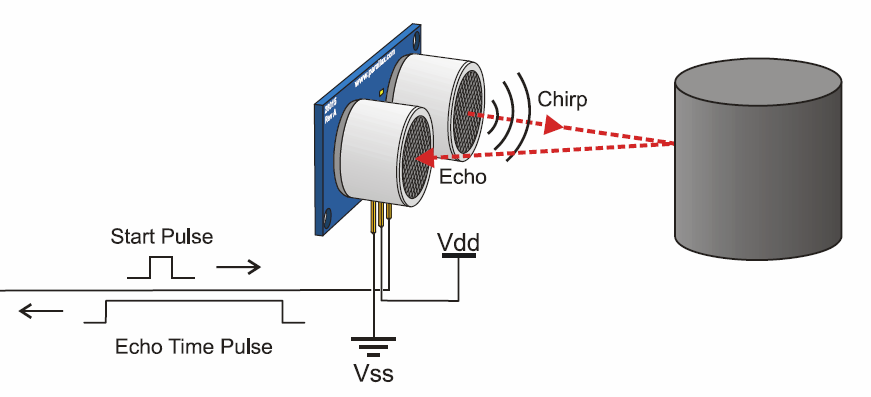
\includegraphics[width=0.7\textwidth]{fig/dsensor}
  \caption{Ultrasonic range sensor. From \cite{maker}}
  \label{fig:dsensor}
\end{figure}

The distance is calculated as follows:
\begin{align}
	speed = \frac{distance}{time}
\end{align}
In dry air at 20 C, the speed of sound is 343 meters per second \cite{sos}. The equation will give the total distance traveled by the sound pulse, so it must be divided by two. Giving:
\begin{align*}
	distance = \frac{speed \times time}{2}\\
    distance = 17150 \times time \quad [cm] 
\end{align*}

\newpage

\subsection{Image Sensor}
The image sensor is one of the most important components in the system. There are several different types of image sensors available, but most of the image sensors I will use consist of an array of small sensors capable of detecting incoming illumination energy and transforming it to digital images.\\

Gonzales explains the process of the digital image sensor as follows: \emph{"The idea is simple: Incoming energy is transformed into a voltage by the combination of input electrical power and sensor material that is responsive to the particular type of energy (wavelength) being detected. The output voltage waveform is the response of the sensors, and a digital quantity is obtained from each sensor by digitizing its response."}\cite{g}\\

That means the response of each sensor in the sensor array of the image sensor is a continuous voltage waveform, and to create digital images from this data the process of sampling and quantization must be applied. Figure \ref{fig:sample} illustrates the the basic idea behind sampling and quantization.
\begin{figure}[h]
  \centering
  \captionsetup{justification=centering}
  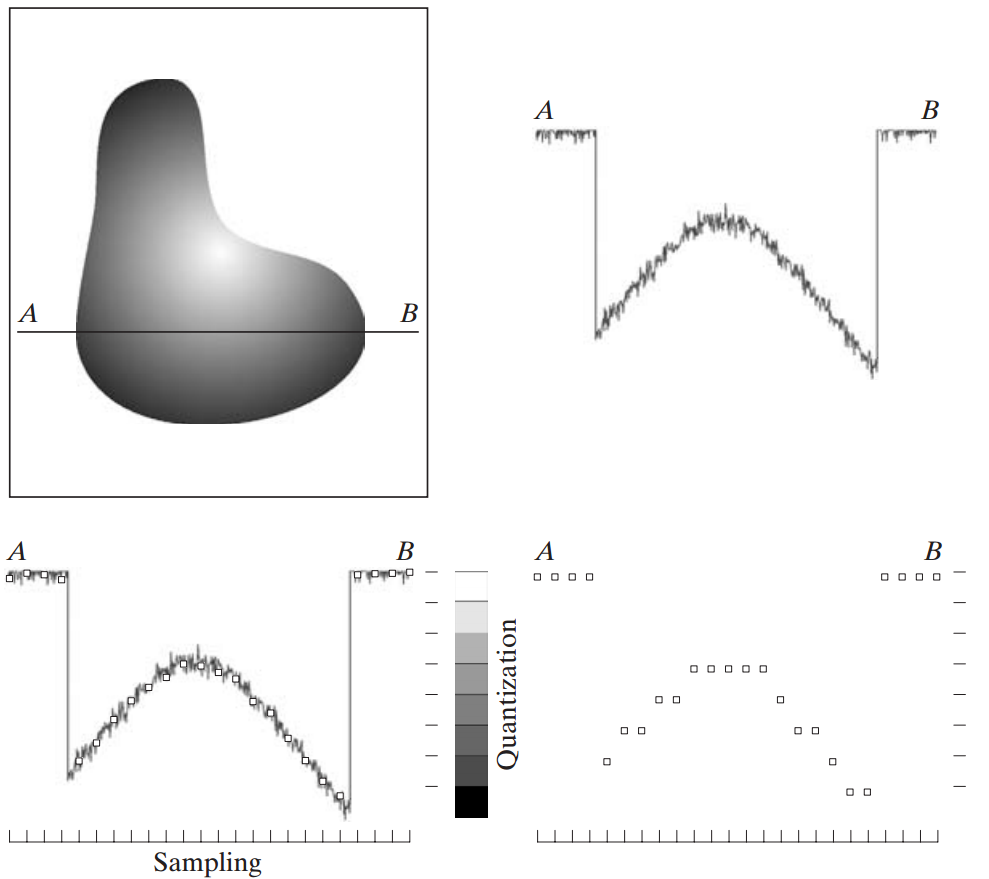
\includegraphics[width=0.7\textwidth]{fig/sample}
  \caption{ Top left: Continuous image\\
  Top right: A scan from A to B in the continuous image\\
  Bottom left: Sampling and quantization\\
  Bottom right: Digital scan line \cite{g}}
  \label{fig:sample}
\end{figure}

Sampling can be described as digitizing the coordinate values of the image, while quantization is the process of digitizing the amplitude values in the image. The amplitude of any given coordinate in the detected image is the intensity value. In terms of our application, it is not vital to understand every detail of how the image sensor works, but a general understanding of the technology is preferred.\\

The image sensor used in this thesis is the IMX219, which is a active pixel sensor CMOS (APS CMOS) image sensor using CMOS technology. APS means that the integrated circuit in the sensor contains an array of pixel sensors, where each pixel contains a photodetector and amplifier.

\begin{figure}[h]
  \centering
  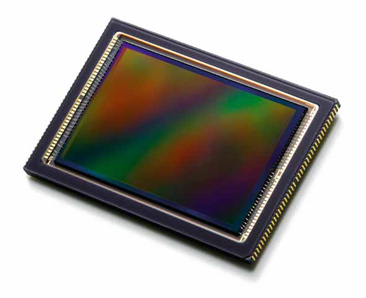
\includegraphics[width=0.4\textwidth]{fig/cmos}
  \caption{APS CMOS Image Sensor}
  \label{fig:cmos}
\end{figure}

Figure \ref{fig:cmos} depicts an APS CMOS image sensor. CMOS is one of the leading technologies for small image sensors often used in mobile phone cameras. CMOS is a technology for designing integrated circuits, and is preferred in image sensors for its small power consumption and small image lag. \\





\newpage
\subsection{Technical hardware requirements}
If a complete image processing algorithm is to be implemented on a mobile computation device, the hardware selected needs to be able to compute and run image processing in a timely manner. Image processing is known to be demanding on hardware, and most advanced implementations such as autonomous cars use high-end dedicated graphic cards \cite{tesla} to be able to run in real time. The algorithm I am implementing does not map in real time, thus the requirements for our hardware performance is reduced. Our hardware should feature enough processing power and storage to be able to run the image processing algorithm as well as storing the image in between operations.\\

These are some of the over-arching hardware requirements:
\begin{itemize}
\item Capable of convolving high resolution images ($>1920\times1080$ pixels)
\item Enough RAM to store images during operations
\item Dedicated graphics chip
\item Powerful enough to be suitable for further project developments into real-time
\end{itemize}

The size of the image output is maximum $3280 \times 2464 $, which makes approximately 8.08M pixels. Since the bit depth of the sensor is 10-bit, I can calculate the file size of the image:

\begin{align*}
3280\times 2464 \quad[pixels] \times 10[bit] = 80819200\quad[bit] = 10102400\quad[bytes]\\
10102400\quad[bytes] \div1048576 = 9,63\quad[Megabytes]
\end{align*}

I assume the image file size is at a maximum $10$ Megabytes for calculation purposes. This means that the hardware needs to provide sufficient RAM to store images of several Megabytes. The GPU should also be able to do operations on pictures of this size, which means a dedicated graphics chip could be beneficial to the system.

%Litt mer

\newpage
\subsection{Positioning of the system}
In the problem description of this paper, the following is stated:
\begin{center}
\emph{"Determine how information such as attitude, height and position can be extracted from the drone, and what the difficulties are with respect to the accuracy of this information"}
\end{center}

There are several potential solutions available to be able to extract useful positional data from a drone. The determining factor in positioning is its accuracy, and if the positioning needs to be indoors or outdoors. 

\subsubsection{Pure IMU based positioning}
This is the most simple and cheapest potential solution to positioning. One would think using an inertial measurement unit (IMU) some useful information about position could be extracted, but this is rarely the case.\\

IMU works great when measuring orientation, this is because it uses a gyroscope to measure linear velocity, and integrate it once to get orientation. There is some linear drift in there, but since I can measure the magnetic north and the gravity vector, it can be corrected for.\\

This not true for positional tracking. In order to track the position, the accelerometers needs to be used to measure acceleration, as opposed to linear velocity. The acceleration needs to be integrated twice to get the position. And thus the big issue occurs when integrating twice, since you are not accumulating error in the linear fashion, but in the quadratic fashion. That means the drift will always increase, thus making it not suitable for positioning.\cite{robot}\\

During the initial phases of this paper, a meeting was conducted with a researcher at the  Department of Engineering Cybernetics together with my advisor. The researcher confirmed the fact that IMU positioning is not feasible for the paper, and that other avenues should be evaluated.

\subsubsection{GPS positioning}
If the drone is designed to operate outdoors, GPS positioning is a great way to control the drone. GPS positioning is the most commercially technology available in autopilots for drones, and is used in many different applications. One major disadvantage in this technology is that it performs poorly indoors, thus making it only accurate for outdoor use.\\

By the use of triangulation between at least three satellites, the position can be extracted in three dimensions. GPS chips are available in very small sizes and range from very cheap off-the shelf hardware to expensive dedicated GPS with high accuracy.\\

Many drone autopilots feature a built-in GPS chip that provides position relatively accurate, making the operator able to control the drones position. The system which I am working on is meant to be used indoors, so GPS positioning would not be a good solution to the positioning needs of the system.

\subsubsection{Camera assisted indoor positioning}
Camera assisted positioning can be many things, but what I mean by this is an array of cameras providing positioning by detecting an element in the images captured by the cameras. A system similar to this is implemented on NTNU in the B333 "Bevegelseslab" room in the Electronics Department.\\

The system works by having several cameras placed at different locations in a room detect an object from different angles, and then place this object in a 3D reference frame in relation to a coordinate system selected by the user by triangulation. This system provides a very accurate position estimate, as well as a very accurate orientation estimate, but is often very expensive to implement because of the hardware required.\\

In most cases, such a system is used for testing purposes, where a position- or orientation estimator is compared to the position and orientation provided by the camera system. This is because the camera system will provide a very accurate position in three dimensions.


















